\chapter{Problem kliki}

\section{Wstęp}

Kliką nazywamy taki podzbiór wierzchołków $V'$ ze zbioru $V$, że występujące w nim wszystkie wierzchołki są połączone między sobą krawędziami. Jeżeli moc zbioru $| V' | = k$  to mówimy że klika jest rozmiaru $k$, oczywiście każdy graf pełny $K_{n}$  jest kliką rozmiaru $n$.

\section{Przedstawienie problemu}

Problem maksymalnej kliki (CLIQUE) polega na znalezieniu w grafie nieskierowanym $G$ kliki o największym rozmiarze.


\begin{twr}
CLIQUE $\in$ NP-zupełnych.
\end{twr}

\section{Dowód przez redukcje}
\begin{proof}
Sprawdzenie, że problemu CLIQUE należy do klasy NP odbywa się poprzez sprawdzenie podzbioru V'[zawarty bądź równy] V będącego świadectwem. Jeśli w podzbiorze V' między każdą parą wierzchołków występuje krawędź to oznacza to że tworzą one klikę. Taki algorytm sprawdzający wykonuje dokładnie  $teta - o zkreska(n) = n^2$ operacji dla każdego wierzchołka, czyli jest złożoności wielomianowej. Dowodzi to że CLIQUE [należy do] NP.

Kolejnym krokiem dowodu jest pokazanie że problem CLIQUE jest Np-trudny. Aby tego dokonać wykorzystam fakt że problem 3-CNF jest NP-zupełny. Problem 3-CNF jest formułą logiczną zawierającą klauze połączone koniunkcją, natomiast każda klauzula składa się z dokładnie trzech literałów połączonych alternatywą. Zadanie polega na znalezieniu takich wartościowań literałów dzięki których formuła jest spełniana. 

Przedstawię teraz sposób sprowadzenia problemu 3-CNP do problemu znalezienia kliki w grafie. Każda klauzula będzie określała oddzielną grupę wierzchołków, a w każdej z nich będą się znajdowały dokładnie trzy wierzchołki odpowiadające konkretnym literałom. Krawędzią połączymy te wierzchołki które spełniają jednocześnie dwa warunki:
- wierzchołki nie należą do wspólnej klauzuli
- literały odpowiadające wierzchołkom nie są sprzeczne.
 Szukać będziemy takiej kliki która połączy ze sobą wszystkie klauzule. Jak łatwo zauważyć transformacja egzemplarza 3-CNF na egzemplarz grafowy można bez większych problemów wykonać w czasie wielomianowym.

Przyjrzyjmy się teraz związkowi jaki tworzą między sobą te dwa zadania. Nie połączyliśmy ze sobą wierzchołków w tej samej klauzuli co oznacza że wystarczy że znajdziemy tylko jeden literał prawdziwy, co sprawi że dzięki wewnętrznym alternatywą cała klauzula będzie prawdziwa. Łączymy ze sobą tylko nie sprzeczne literały co oznacza że zmienne nie mogą jednocześnie posiadać dwóch różnych wartości. Zbierając to wszystko do siebie chcę pokazać że znalezienie kliki na tych klauzulach oznacza znalezienie niesprzecznych wartości literałów które w rezultacie spełniają całą formułę. Natomiast z drugiej strony znalezienie wartościowań literałów pozwalających uczynić formułę spełnialną oznacza że w takiej konstrukcji grafu musi istnieć klika wielkości liczbie klauzul w formule.  



------------------------------------------

Świadectwem dla problemu CLIQUE jest podzbiór wierzchołków $V'$ zawierających klikę. Aby sprawdzić autentyczność tego świadectwa wystarczy jedynie sprawdzić, czy dla każdej pary wierzchołków z tego podzbioru istnieje krawędź. To sprawdzenie ma złożoność kwadratową, czyli wielomianową.

Aby pokazać, że CLIQUE jest NP-trudny podeprzemy się faktem że problem 3-CNF jest NP-trudny i przedstawię redukcje 3-CNF [$<=$] p CLIQUE. [kolki = C1 i C2 i ... Ck] oznaczmy jak formułę problemu 3-CNF składającą się z $r = 1,2,...k$ klauzul. Na każdą klauzulę składają się dokładnie 3 literały $l^r,1, l^r,2, l^r,3$. Skonstruujemy graf $G$ z formuły [kolko] w ten sposób że formuła jest spełniana wtedy i tylko wtedy, gdy G zawiera klikę o rozmiarze k.


... redukcja z 3CNF

\begin{figure}[tbh]
PRZYKLAD
\centering

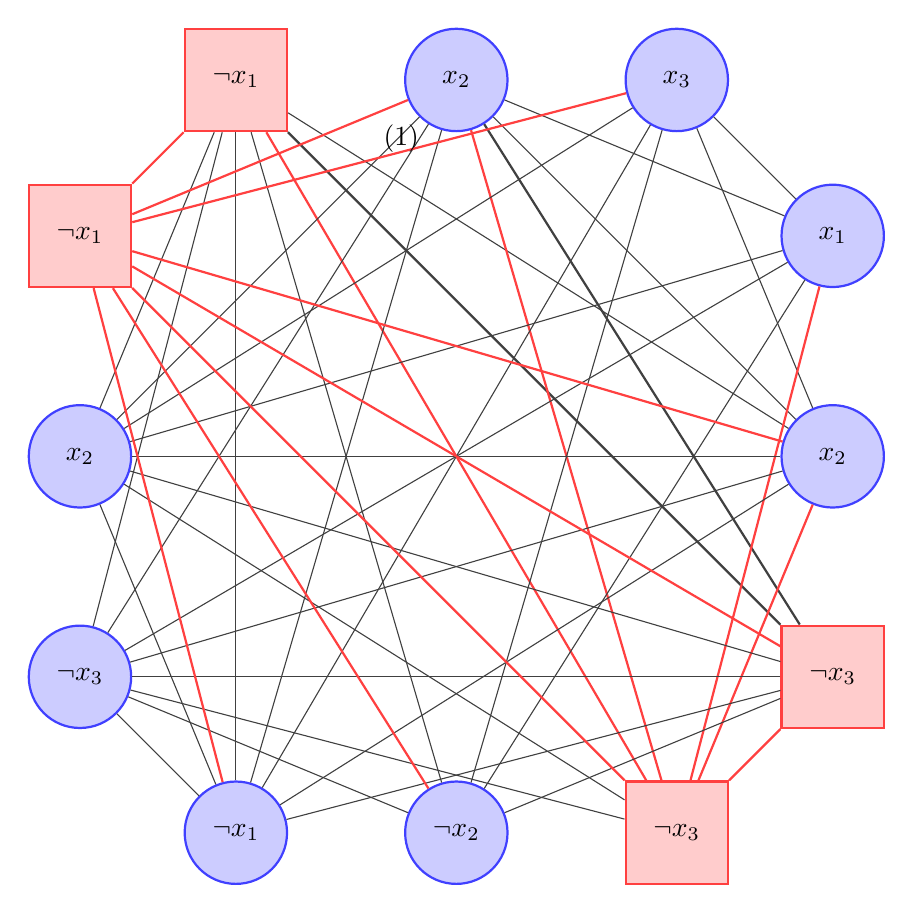
\begin{tikzpicture} [node distance=2.8cm]

\tikzstyle{unmark_vertex}=[circle,thick,draw=blue!75,fill=blue!20,minimum size=13mm]
\tikzstyle{mark_vertex}=[rectangle,thick,draw=red!75,
  			  fill=red!20,minimum size=13mm]
\tikzstyle{mark_edge}=[thick,draw=red!75]
\tikzstyle{unmark_edge}=[draw=black!75]

  \begin{scope}
  	\node [mark_vertex] (c1v1) {$\neg{x}_{1}$};
  	\node [unmark_vertex] (c1v2) [right of=c1v1] {${x}_{2}$};
  	\node [unmark_vertex] (c1v3) [right of=c1v2] {${x}_{3}$};
  	
  	\node [unmark_vertex] (c2v1) [below right of=c1v3] {${x}_{1}$}
  		[unmark_edge] edge (c1v2)
  		[unmark_edge] edge (c1v3);
  	\node [unmark_vertex] (c2v2) [below of=c2v1] {${x}_{2}$}
  		[unmark_edge] edge (c1v1)
  		[unmark_edge] edge (c1v2)
  		[unmark_edge] edge (c1v3);
  	\node [mark_vertex] (c2v3) [below of=c2v2] {$\neg{x}_{3}$}
  		[mark_edge] edge (c1v1)
  		[unmark_edge] edge (c1v2);
  	
  	\node [mark_vertex] (c3v3) [below left of=c2v3] {$\neg{x}_{3}$}
  		[mark_edge] edge (c1v1)
  		[unmark_edge] edge (c1v2)
  		[unmark_edge] edge (c2v1)
  		[unmark_edge] edge (c2v2)
  		[mark_edge] edge (c2v3);
  	\node [unmark_vertex] (c3v2) [left of=c3v3] {$\neg{x}_{2}$}
  		[unmark_edge] edge (c1v1)
  		[unmark_edge] edge (c1v3)
  		[unmark_edge] edge (c2v1)
  		[unmark_edge] edge (c2v3);
  	\node [unmark_vertex] (c3v1) [left of=c3v2] {$\neg{x}_{1}$}
  		[unmark_edge] edge (c1v1)
  		[unmark_edge] edge (c1v2)
  		[unmark_edge] edge (c1v3)
  		[unmark_edge] edge (c2v2)
  		[unmark_edge] edge (c2v3);
  	
  	\node [unmark_vertex] (c4v3) [above left of=c3v1] {$\neg{x}_{3}$}
  		[unmark_edge] edge (c1v1)
  		[unmark_edge] edge (c1v2)
  		[unmark_edge] edge (c2v1)
  		[unmark_edge] edge (c2v2)
  		[unmark_edge] edge (c2v3)
  		[unmark_edge] edge (c3v1)
  		[unmark_edge] edge (c3v2)
  		[unmark_edge] edge (c3v3);
  	\node [unmark_vertex] (c4v2) [above of=c4v3] {${x}_{2}$}
  		[unmark_edge] edge (c1v1)
  		[unmark_edge] edge (c1v2)
  		[unmark_edge] edge (c1v3)
  		[unmark_edge] edge (c2v1)
  		[unmark_edge] edge (c2v2)
  		[unmark_edge] edge (c2v3)
  		[unmark_edge] edge (c3v1)
  		[unmark_edge] edge (c3v3);
  	\node [mark_vertex] (c4v1) [above of=c4v2] {$\neg{x}_{1}$}
  		[mark_edge] edge (c1v1)
  		[unmark_edge] edge (c1v2)
  		[unmark_edge] edge (c1v3)
  		[unmark_edge] edge (c2v2)
  		[mark_edge] edge (c2v3)
  		[unmark_edge] edge (c3v1)
  		[unmark_edge] edge (c3v2)
  		[mark_edge] edge (c3v3);

	\node at (2.1cm, -0.75cm) {\text{(1)}};
  \end{scope}
  
  
\end{tikzpicture}

\caption{Przykład wykonania algorytmu VERTEX-COVER-EDGES-APPROX. Przykład przedstawia model prezentujący formułę 3-CNF [ozkreską = C1 i C2 i C3 i C4], C1 = nx1 lub x2 lub x3, C2= x1 lub x2 lub nx3, C3 = nx1 lub nx2 lub nx3, C4 = nx1 lub x2 lub nx3 w postaci grafu G problemu CLIQUE. Dla tak określonej formuły wartościowanie x1 = 0, x3 = 0 spełnia formułe, natomiast zmienna x2 pozostaje dowolna. Na grafie jest to zobrazowane czerwonymi wierzchołkami zawierajacymi klikę. }
\label{vertex-cover-edges-approx_example}

zakomentarzowany tekst
\end{figure}

koniec
\end{proof}


\section{Algorytm aproksymacyjny}

Dzięki temu że problem CLIQUE jest dualny do problemu VERTEX-COVER, to algorytmy z poprzedniego rozdziału również po odpowiednim przeformułowaniu wejścia zwracają rozwiązania problemu CLIQUE